\documentclass[]{article}
\usepackage[utf8]{inputenc}
\usepackage[margin=1.0in]{geometry}
\usepackage{amsmath, amsfonts}
\usepackage{tikz}
\usepackage[english]{babel}
\usepackage{amsthm}
\usepackage{enumitem}
\usepackage{graphicx}
\usepackage{float}
\usepackage[backend=biber]{biblatex}
\usepackage{hyperref}
\usepackage{subcaption}

\newtheorem{theorem}{Theorem}
\newtheorem{definition}{Definition}
\newtheorem{lemma}{Lemma}
\newtheorem{corollary}{Corollary}[theorem]
\renewcommand{\theenumi}{\Alph{enumi}}

\newcommand{\bd}{\textbf}
\newcommand{\del}{\nabla}
\newcommand{\by}{\times}
\newcommand{\trace}{\mathrm{trace}}
\newcommand{\range}{\mathrm{range}}
\newcommand{\R}{\mathbb R}
\newcommand{\C}{\mathbb C}
\newcommand{\M}{\mathcal M}
\newcommand{\Borel}{\mathcal B_{\mathbb R}}
\newcommand{\dprime}{^{\prime\prime}}
\newcommand{\tprime}{^{\prime\prime\prime}}
\newcommand{\x}{\mathbf x}
\newcommand{\y}{\mathbf y}
\newcommand{\z}{\mathbf z}
\renewcommand{\v}{\mathbf v}
\renewcommand{\S}{\mathbb S}
\renewcommand{\u}{\mathbf u}
\newcommand{\innerprod}[2]{\left\langle #1\,, #2 \right\rangle}
\addbibresource{bibliography}


\title{Additional Proofs to Kirsch and Grinberg's  "The Factorization Method for Inverse Problems"}
\date{}
\author{Kale Stahl \\ \small Advised by Dinh-Liem Nguyen and Trung Truong}

\begin{document}
		
		%Makes fancy title
		\makeatletter
		\begin{center}
			{\centering \Large \bd \@title}\\
			\vspace{.5cm}
			{\large \@author}
			\vspace{.25cm}
		\end{center}
		\makeatother
		\begin{abstract}
			The goal of this project is to provide additional proof and explanation of the factorization of the far-field operator for the inverse scattering problem. We seek to prove that the far field operator can indeed be factored into an auxiliary and Herglotz operator. We will then prove that utilizing this factorization yields a unique solution to the inverse scattering problem and implement this method numerically.
		\end{abstract}
		\section{Introduction}		
			This project will be devoted to studying the Factorization method for inverse scattering problems proposed in [\cite{kirschgrinberg2008}] by Kirsch and Grinberg. It will focus on the simplest cases seen in the first chapter of this book. We will consider the scattering of time-harmonic plane waves by an object $D$ which is modeled by the Dirichlet boundary condition on the boundary $\Gamma = \partial D$ of $D$. We consider acoustic waves, which are characterized by the Helmholtz equation. We will omit analysis of the direct scattering problem, and focus only on additional analysis to the factorization methods used to solve the inverse scattering problem for shape identification of the scattering object. We will first show that the far field operator can be decomposed into the solution operator, and then we will prove the factorization of the far field operator. Once this is done, we will prove the uniqueness of the inverse problem utilizing properties of the factorization method and implement the method numerically.
		\section{The Factorization Method}
			It will be within this section that we prove the factorization of the far-field operator $F$. It is the goal of the Factorization method to relate the range of $G$, the solution operator, to $F$. We will first discuss these operators in more detail, and prove an important theorem that allows us to finally decompose $F$ in terms of $G$ and an auxiliary operator $H$.
			\subsection{The Far-Field and Solution Operators}
				We begin by defining the far-field pattern of our field $u$ as follows:
				\begin{definition}\label{def:far-field pattern}
					Let $u \in C^2(\R^3\setminus \overline D)\cap C(\R^3 \setminus D)$ be a radiating solution of the Helmholtz equation such that $u$ possesses a normal derivative on the boundary $\Gamma$. Then $u$ is analytic in $\R^3\setminus\overline D$ and has asymptotic behavior
					\begin{equation} \label{eq:far-field pattern}
						u(x) = \frac{e^{ik|x|}}{4\pi |x|} u^\infty(\hat x) + \mathcal O\left(1/|x|^2\right), \qquad |x|\to \infty
					\end{equation}
					uniformly with respect to $\hat x = x/|x|$. Then we can see the function $u^\infty:\S^2 \to \C$ is analytic and called the \bd{far-field pattern} of $u$. It has the form
					\begin{equation}
						u^\infty(\hat x) = \int\limits_\Gamma\left[u(y)\frac{\partial }{\partial u(y)}e^{-ik\hat x\cdot y} - \frac{\partial u(y)}{\partial u}e^{-ik\hat x\cdot y}\right]\, ds(y) \qquad \hat x\in \S^2 
					\end{equation}
				\end{definition}
				The far-field pattern is essential in proving the uniqueness of the inverse scattering problem seen in Theorem \ref{theorem:uniqueness}. The far-field pattern exists for both the incident field $u^i$ and the scattered wave $u^s$. The far-field pattern for $u^s$ is dependent on both angular coordinate values $\hat x$ and $\theta$ so we will write $u^\infty = u^\infty(\hat x, \theta)$. This pattern defines the far-field operator $F$ as follows:
				\begin{definition}\label{def:F}
					Define the \bd{far-field operator} $F:L^2(\mathbb S^2) \to L^2(\mathbb S^2)$ as
					\begin{equation}	
						(Fg)(\hat x) = \int\limits_{\mathbb S^2}u^\infty(\hat x, \theta)g(\theta)\, ds(\theta) \qquad \hat x\in \S^2
					\end{equation}
					where $u^\infty(\hat x)$ is the far field pattern of $u$ defined in Definition \ref{def:far-field pattern}.

				\end{definition}
				This operator is compact in $L^2(\S^2)$ and contains the known data for the inverse scattering problem. We wish to collect characterization about the shape of our scattering domain $D$ by using $F$. Before we can do this, we need to define an operator $G$.
				\begin{definition}\label{def:G}
					Let the \bd{data-to-pattern operator} $G: H^{1/2}(\Gamma)\to L^2(\S^2)$ be defined by $Gf = u^\infty$ where $u^\infty \in L^2(\S^2)$ is the far field pattern of the solution $u$ to the exterior Dirichlet problem with boundary data $f\in H^{1/2}(\Gamma)$, meaning that $v\in H^1_{\text{loc}}(\R^3\setminus\bar D)$ solves 
					\begin{equation}
						\begin{cases}
							\Delta u + k^2u = 0 &\text{outside }D \\
							u = f & \text{on } \Gamma
						\end{cases}
					\end{equation}
					and 
					\begin{equation}\label{eq:radiation condition}
						\frac{\partial u}{\partial r} - ikv = \mathcal O(r^{-2}) \text{ for } r = |x| \to \infty
					\end{equation}
					uniformly with respect to $\hat x$.
				\end{definition}				
				This operator is compact and injective in $L^2(\S^2)$ and by relating its range to $F$, we can come about a unique characterization for $D$. Before that, we define an auxiliary operator as follows:
				\begin{definition}\label{def:H}
					Define $H: L^2(\mathbb S^2) \to H^{1/2}$ as
					\begin{equation}
						-(Hg)(\hat x) = -\int\limits_{\mathbb S^2}g(\theta)e^{ikx\cdot \theta}\,ds(\theta) \qquad x\in \Gamma
					\end{equation}
					note that this is the trace on $\Gamma$ of the Herglotz wave function with density $g$.
				\end{definition}
				Using these definitions, we will prove the following theorem involving the elementary factorization of the far-field operator into the data-to-pattern operator $G$ and the auxiliary operator $H$.
				\begin{theorem}\label{theorem:theorem1}
					Let $F$ be the far-field operator from Definition \ref{def:F}, $H$ be the auxiliary operator in Definition \ref{def:H}, and $G$ to be the data-to pattern operator in Definition \ref{def:G}. We then arrive at the following factorization of $F$:
					\begin{equation}
						Fg = -GHg
					\end{equation}
				\end{theorem}
				\begin{proof}
					First, take some boundary data in a fixed direction $\theta$, $f_\theta(x)= -e^{ik\theta \cdot x}$. Then by Definition \ref{def:G} we know
					\begin{equation}
						Gf_\theta(x) = u^\infty(\hat x, \theta)
					\end{equation}
					Taking the definition of $H$ and applying to it the solution operator $G$, we have 
					\begin{align}
						(GHg)(x) &= G\int\limits_{\mathbb S^2} g(\theta)e^{ikx\cdot \theta}\,ds(\theta)=  \int\limits_{\mathbb S^2}u^\infty(\hat x, \theta)g(\theta)\, ds(\theta)= -Fg
					\end{align}
					This is what we wished to show, however it is not clear whether we can exchange $G$ and the integral. To do this, we first decompose $f_\theta$ into $f_\theta^+$ and $f_\theta^-$ such that $f_\theta = f_\theta^+-f_\theta^-$ and $f_\theta^+$ and $f_\theta^-$ are positive semi-definite. This is to say that $f^+$ is equal to $f$ on regions where $f>0$ and 0 otherwise, and $f^-$ is equal to $f$ on regions where $f<0$ and 0 otherwise. Since both  $f_\theta^+$ and $f_\theta^-$ are positive functions, we know that there exists a monotone increasing sequence of positive simple functions $\{(f^+_\theta)_{n}\}$ such that $(f^+_\theta)_{n}\to f^+$ as $n \to \infty$. We can write each term in this sequence as $f^+_{n} = \sum^n_{i=0}\alpha_i(x)\chi_{E_i}(\theta)$.
					
					Each $\alpha_i$ is a constant and $\chi_{E_i}$ are characteristic functions of some set $E_i$ such that $\bigcup_{i = 0}^\infty E_i = \S^2$. Thus, by the summation definition of the Lebesgue integral, we see that the $G$ operator can be exchanged with the integral. By the Monotone Convergence theorem, we can take the limit as $n\to \infty$ and again exchange the integral and limit. We can apply the same reasoning to $f_\theta^-$ by the linearity of the Lebesgue integral. So then with this shown, we indeed have 
					\begin{equation}
						Fg = -GHg 
					\end{equation}
					and we are finished.
				\end{proof}
			\subsection{Factorization of the Far-Field Operator}
				Now that we have shown a factorization of $F$ in terms of $G$, we wish to factorize further, writing the difficult to work with $G$ in terms of simpler operators. To do this, we define another operator $S$.
				\begin{definition} \label{def:S}
					Define the \bd{single layer boundary operator} $S : H^{-1/2}(\Gamma) \to H^{1/2(\Gamma)}$ by
					\begin{equation}
						S\varphi(x) := \int\limits_\Gamma \Phi(x, y) \varphi(y)\, ds(y), \qquad x \in \Gamma
					\end{equation}
					with 
					\begin{equation}\label{eq:green's function}
						\Phi(x, y) = \frac{e^{ik|x-y|}}{4\pi|x-y|}, \qquad x, y \in \R^3, \quad x\neq y
					\end{equation}
					which is the fundamental solution the the Helmholtz equation in three dimensions.
				\end{definition}
				This operator has unique qualities that lend itself nicely in the inverse problem, the largest being shown in the following Lemma.
				\begin{lemma} \label{lemma:solution}
					$v= S\varphi$ is a solution to the Helmholtz equation. Moreover, $H^\ast \varphi$ is equal to the far-field pattern, $v^\infty$, for $v$.
				\end{lemma}
				\begin{proof}
					This proof will proceed in three main steps. In the first, we will show that $v$ is a solution to the Helmholtz equation. We will then show that it satisfies the necessary radiation condition in (\ref{eq:radiation condition}), and finally we will show that indeed $H^\ast \varphi = v^\infty$
					
					We begin by taking $\Phi$ as defined in (\ref{eq:green's function}). Since this is the fundamental solution to the Helmholtz equation, for some fixed $y\neq x$, we have the following:
					\begin{equation}
						\Delta_x \Phi(x, y) + k^2 \Phi(x, y) = \delta(x-y)
					\end{equation}
					We can multiply both sides by $\varphi(y)$ and integrate over $\partial D$ to see
					\begin{equation} \label{eq:14}
						\int\limits_{\partial D}\Delta_x \Phi(x, y)\varphi(y) + k^2 \Phi(x, y)\varphi(y)\, ds(y) = \int\limits_{\partial D}\delta(x-y)\varphi(y)\, ds(y)
					\end{equation}
					Since $x\neq y$, the right-hand side of (\ref{eq:14}) goes to 0. We see
					\begin{equation}
						\int\limits_{\partial D}\Delta_x \Phi(x, y)\varphi(y)\, ds(y) + k^2\int\limits_{\partial D}\Phi(x, y)\varphi(y)\, ds(y) = 0
					\end{equation}
					By the linearity of the Lebesgue integral, and the fact that $\Delta_x$ does not depend on the variable of integration, we are able to exchange the order of it and the integral. To prove that this is indeed permissible, we first consider the limit definition of the derivatives included in the $\Delta_x$ operator. Considering a single derivative with respect to $x_1$ we have
					\begin{equation}
						\frac{\partial }{\partial x}\Phi(x, y) = \lim_{(\delta x_1)_n \to 0}\frac{\Phi(x+ (\delta x_1)_n, y) - \Phi(x, y)}{(\delta x_1)_n}
					\end{equation}
					Define $(\delta x_1)_n = \frac{1}{n}$ so that $(\delta x_1)_n\to 0 $ as $n \to \infty$. We will now apply Lesbesgue's Dominated Convergence theorem. We first note that $ \left|\frac{\Phi(x+ (\delta x_1)_n, y) - \Phi(x, y)}{(\delta x_1)_n}\right|$ is bounded from above by $|\Phi(x, y)|$ which is in $L^2(\partial D)$. Thus, by the Dominated Convergence Theorem we have
					\begin{equation}
						\int\limits_{\partial D}\frac{\partial }{\partial x_1}\Phi(x, y)\, ds(y) = \int\limits_{\partial D}\lim_{(\delta x_1)_n \to 0}\frac{\Phi(x+ \delta x_n, y) - \Phi(x, y)}{\delta x_n}\, ds(y) =  \frac{\partial }{\partial x_1}\int\limits_{\partial D}\Phi(x, y)\, ds(y)
					\end{equation}
					The same argument can be repeated for both the second derivative of $x_1$ and the two derivatives of $x_2$, meaning the entire $\Delta_x$ operator can be exchanged with the integral.
					Finally, by applying Definition \ref{def:S}, we see that
					\begin{equation}
						\Delta_xS\varphi(x)+ k^2\, S\varphi(x) = 0
					\end{equation}
					Meaning that $v = S\varphi(x)$ is indeed a solution to the Helmholtz equation.				
					
					Next we will show that $v = S\varphi(x)$ satisfies the necessary radiation condition. We note that our radiation condition is given by (\ref{eq:radiation condition}).	By applying the radiation condition to $\Phi (x, y)$, we see
					\begin{equation}
						\frac{\partial}{\partial |x|}\Phi (x, y) - ik \Phi (x, y) = \mathcal O(|x|^{-2})
					\end{equation}
					Similarly to above, we can multiply both sides by $\varphi(y)$ and integrate over $\partial D$. We see
					\begin{equation}
						\int_{\partial D}\frac{\partial}{\partial |x|}\Phi (x, y)\varphi(y)\, ds(y) - \int_{\partial D}ik \Phi (x, y)\varphi(y)\, ds(y) = \int_{\partial D}\mathcal O(|x|^{-2})\, ds(y)
					\end{equation}
					By the same argument used previously, we can exchange the order of the derivative and integral, seeing
					\begin{equation} \label{eq:21}
						\frac{\partial}{\partial r}S\varphi(x) - ikS\varphi(x) = \mathcal O(|x|^{-2})
					\end{equation}
					The right-hand side of (\ref{eq:21}) will go to zero as the integral is over the boundary and any small terms will vanish. Thus, $v= S\varphi(y)$ satisfies our radiation condition.
					
					Finally we will show that $H^\ast \varphi$ is the far-field pattern of $v$. By Definition \ref{def:far-field pattern}, we can calculate the far-field pattern of $\Phi$ to be given by
					\begin{equation}
						\Phi^\infty(\hat x, y) = e^{-ik\hat x\cdot y}
					\end{equation}
					We then see that by applying (\ref{eq:far-field pattern}) to $v =S\varphi$, we have 
					\begin{align}
						S\varphi(\hat x) &= \frac{e^{ik|x|}}{|x|}\left[ (S\varphi)^\infty(\hat x) + \mathcal O(|x|^{-2})\right] \\
						&= \int\limits_{\partial D}\frac{e^{ik|x|}}{|x|}\left[ \Phi^\infty(\hat x, y) + \mathcal O(|x|^{-2})\right] \varphi(y)\, ds(y)\\
						&= \frac{e^{ik|x|}}{|x|}\left[ \int\limits_{\partial D} e^{-ik\hat x\cdot y}\varphi(y)\, ds(y) + \mathcal O(|x|^{-2})\right] \\
						&= \frac{e^{ik|x|}}{|x|}\left[ H^\ast \varphi(y) + \mathcal O(|x|^{-2})\right] \\
					\end{align}
					From here we can conclude that indeed $	(S\varphi)^\infty(\hat x) =H^\ast \varphi(\hat x)$ and we are finished.
				\end{proof}
				Now that we have a relation between $S$ and $H$, we can arrive at a final factorization of $F$ in terms of only $S$ and $H$. 
				\begin{theorem}
					If $k^2$ is not a Dirichlet Eigenvalue of $-\Delta$ in $D$ we arrive at the following factorization for the far-field operator:
					\begin{equation}
						F = H^\ast S^{-1}H
					\end{equation}
				\end{theorem}
				\begin{proof}
				We will first calculate $H^\ast$ explicitly. We see for some $f \in L^2(\mathbb S^2)$ and $g\in H^{1/2}(\partial D)$ we have the following relationship between inner products:
				\begin{equation}
					\innerprod{Hf}{g}_{H^{1/2}} = \innerprod{f}{H^\ast g}_{L^2}\label{Hstar}
				\end{equation}
				where the inner products are known to be as follows:
				\begin{equation}
					\innerprod{f(x)}{g(x)}_{H^{1/2}(\partial D)} = \int\limits_{\partial D} \overline{g(x)}f(x)\, ds(\theta)
				\end{equation}
				\begin{equation}
					\innerprod{f(x)}{g(x)}_{L^2(\mathbb S^2)} = \int\limits_{\mathbb S^2}\overline{g(x)}f(x)\, ds(\theta)
				\end{equation}
				Using (\ref{Hstar}) we can calculate $H^\ast$, seeing
				\begin{align}
					\innerprod{Hf}{g}_{H^{1/2}} &=  \int\limits_{\partial D} \overline{g(x)}Hf(x)\, ds(\theta)\\
					 &=  \int\limits_{\partial D} \overline{g(x)} \int\limits_{\mathbb S^2}f(\theta)e^{ikx\cdot \theta}\, ds(\theta) \, ds(\theta)\\
					 &=  \int\limits_{\mathbb S^2}\int\limits_{\partial D}  \overline{g(x)e^{-ikx\cdot \theta}}\, ds(\theta)f(\theta) \, ds(\theta)\\
					 &= \innerprod{f}{H^\ast g}_{L^2}
				\end{align}
				So then we have
				\begin{equation}
					H^\ast g(\theta) = \int\limits_{\partial D}g(x)e^{-ikx\cdot \theta}\, ds(\theta)
				\end{equation}
				Now we can see that by Lemma \ref{lemma:solution} we have $H^\ast = GS$. This comes bout by Definition \ref{def:G}, seeing $G(S\varphi) = (S\varphi)^\infty$. Thus we have,
				\begin{equation}
					 -H^\ast S^{-1}Hg = -GSS^{-1}Hg = -GIHg = -GHg
				\end{equation}
				Where $I$ is the identity operator. Then by Theorem \ref{theorem:theorem1} we know that $-GH = F$ and we arrive at
				\begin{equation}
					-H^\ast S^{-1}H = F
				\end{equation} and we are finished.\\
			\end{proof}
		\section{Uniqueness of the Solution to the Factorization Method}
			The following theorem, which appears in [\cite{kirschgrinberg2008}] without proof, is used to prove the uniqueness of the solution to the inverse scattering problem. The proof of the theorem in [\cite{coltonkress2013}] uses more general tools such as Rellich's lemma, but we can utilize what we have already proved about the factorization method along with general notions about the inverse scattering problem to arrive at a rather elegant proof. We also need to establish some general facts about the far-field pattern before we can arrive at this proof. The following Lemma helps to show the relation between the far field pattern and the domain $D$.
			\begin{lemma}\label{lemma:test-function}
				Let $G$ be defined as in Definition \ref{def:G}. For any $z\in \R^3$ define the test function $\phi_z \in L^2(\S^2)$ by 
				\begin{equation}
					\phi_z(\hat x) := e^{-ik\hat x\cdot z}, \qquad \hat x\in \S^2
				\end{equation}
				Then $\phi_z$ belongs to the range of $G$ if and only if $z\in D$.
			\end{lemma}
			\begin{proof}
				We first take some $z\in D$ and define
				\begin{equation}
					v(x) := \Phi(x, z) = \frac{e^{ik|x-z|}}{4\pi |x-z|}, \quad x\notin D
				\end{equation}
				such as in (\ref{eq:green's function}) and some $f|_\Gamma$. Then $f \in H^{1/2}(\Gamma)$. Then the far-field pattern of $v$ is given by 
				\begin{equation}
					v^\infty(\hat x) = e^{-ik\hat x\cdot z}, \hat x \in \S^2
				\end{equation}
				which coincides with $\phi_z$, meaning $Gf = v^\infty = \phi_z$. Thus, $\phi_z$ is in the range of $G$. Now, for the sake of contradiction, suppose that $z \notin D$ and that there exists some $f \in H^{1/2}(\Gamma)$ with $Gf = \phi_z$. Let $v$ be the solution to the exterior Dirichlet problem with boundary data $f$ such that $v^\infty = Gf$ is its far-field pattern. Since $\phi_z$ is the far-field pattern of $\Phi(\cdot, z)$, we can conclude via Rellich's Lemma that $v(x) = \phi(x, z)$ for all $x$ outside of any ball containing $D$ and the point $z$, so they must coincide on $\R^3\setminus(\overline{D}\cup \{z\})$. 
				
				If $z\notin \overline D$, this contradicts the fact that $\Phi(x, z)$ is singular at $x = z$ and the fact that $v$ must be analytic on $\R^3\setminus \overline D$. 
				
				If instead, $z \in \Gamma$, then we have that $\Phi(x, z) = f(x)$ for $x\neq z\in \Gamma$. This would mean that the function $x \mapsto \Phi(x, z)$ is in $H^{1/2}(\Gamma)$. This is a contradiction, as $\nabla \Phi(x, z) = \mathcal O\left( \frac{1}{|x-z|^2}\right)$ in the limit as $x \to z$ meaning that this function cannot be in $H^1(D)$ or $H^1_{loc}(\R^3\setminus \overline D)$. Since $H^{1/2}(\Gamma) = \trace(H^1(D))$, this is a contradiction and the only way for $\phi_z$ to be in the range of $G$ is when $z \in D$.
			\end{proof}
			This allows us to associate a test function with our domain and characterize whether or not a point exists within the domain. With this defined, we can state the following uniqueness theorem:
			\begin{theorem}\label{theorem:uniqueness}
				For a fixed wavenumber $k>0$ the far field patterns $u^\infty(\hat x, \theta)$ uniquely determine the shape of the scattering object $D$. This means that if there are two objects $D_1$ and $D_2$ with corresponding far field patterns $u_1^\infty(\hat x, \theta)$ and $u_2^\infty(\hat x, \theta)$ respectively, then $u_1^\infty(\hat x, \theta)=u_2^\infty(\hat x, \theta)$ implies that $D_1=D_2$.
			\end{theorem}
			\begin{proof}
				To prove this, we first begin by supposing there are two objects, $D_1$ and $D_2$ such that their far-field patterns $u_1^\infty(\hat x, \theta)$ and $u_2^\infty(\hat x, \theta)$ coincide. We can take some $z_1, z_2\in \R^3$ such that $\phi_{z_1}(\hat x) = e^{-ik\hat x \cdot z_1}$ and $\phi_{z_2}(\hat x) = e^{-ik\hat x \cdot z_2}$. By Lemma \ref{lemma:test-function} we know that for some boundary data $f$, that $Gf = \phi_{z_1}$ if and only if $z_1 \in D_1$. Then we know by Definition \ref{def:G} that $\phi_{z_1}$ must coincide with the far-field pattern of $D_1$ for all points $z_1 \in D_1$. Since $u_1^\infty(\hat x, \theta)$ and $u_2^\infty(\hat x, \theta)$ are the same, we can conclude that $\phi_{z_1}$ also coincides with $u_2^\infty(\hat x, \theta)$ for all points $z_1\in D_1$. We then reason that $\phi_{z_1} = \phi_{z_2}$ for all $z_1\in D_1$. This implies that $D_1 \subseteq D_2$. We can use exactly the same reasoning for the reverse inclusion $D_2 \subseteq D_1$, and we see that indeed $D_1 = D_2$.
			\end{proof}
		\section{Numeric Simulations}
			This section will show the Factorization Method implemented with simulated data and its ability to reconstruct various objects. MATLAB code samples for implementing the factorization method are found in \cite{potthast2015}. The code used to create these simulations can be found on my \href{https://github.com/KaleStahl/Honors-Project}{Github}.
			\subsection{Noiseless Data}
				 We begin by taking three differently shaped scattering objects and use the factorization method to reconstruct them. In Figure \ref{fig:noiseless}, we have a kite, a circle, and an ellipse.
				\begin{figure}[h]
					\centering
					\begin{subfigure}{.3\textwidth}
						\centering
						\includegraphics[width = \textwidth]{Numeric Simulations/Images/Circle-Reconstructed}
						\caption{Circle shaped scattering object}
					\end{subfigure}
					\begin{subfigure}{.3\textwidth}
						\centering
						\includegraphics[width = \textwidth]{Numeric Simulations/Images/ellipse-Reconstructed}
						\caption{Ellipse shaped scattering object}
					\end{subfigure}
					\begin{subfigure}{.3\textwidth}
						\centering
						\includegraphics[width = \textwidth]{Numeric Simulations/Images/kite-Reconstructed}
						\caption{Kite shaped scattering object}
					\end{subfigure}
					\caption{Reconstructions of scattering objects with no noise in data.}
					\label{fig:noiseless}
				\end{figure} 
				We can see that the reconstructions are rather accurate. The reconstructions in Figure \ref{fig:noiseless} have data which is has no "noise", that is, the data used to reconstruct the object is representative of the exact data expected from the scattering problem.
			
			\subsection{Noisy Data}
				In practical applications this is not always the most feasible assumption, as real data is often "noisy". This noise can be caused by various factors, but yields data which varies from the expected perfect data. To simulate this, we will add randomly generated Gaussian noise to the far-field operator used to solve the inverse problem. This noise is scaled such that the matrix norm of the noisy far-field operator and the exact far-field operator differ by a given percent, which we will represent our "noise level" in the figures. The estimate used in the noise generation technique to do this is found in \cite{hansen1988}. We see in Figure \ref{fig:circlenoise} circles, in Figure \ref{fig:ellipsenoise} ellipses, and Figure \ref{fig:kitenoise} kites, all with various levels of noise. Obviously the reconstructions are much less accurate than their noiseless counterparts, but they are still able to reconstruct the general shape of the original object.
				\begin{figure}[h]
					\centering
					\begin{subfigure}{.3\textwidth}
						\centering
						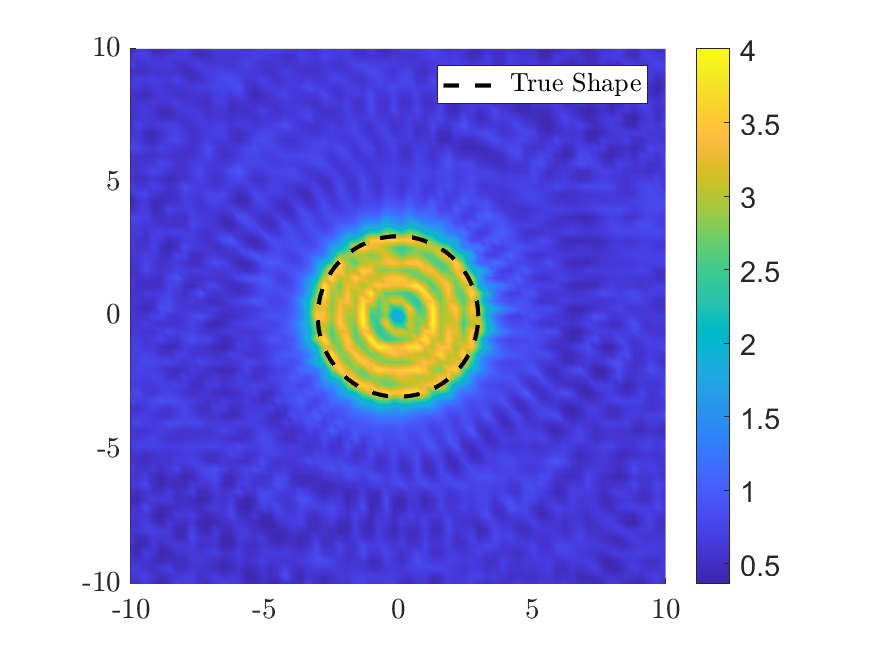
\includegraphics[width = \textwidth]{Numeric Simulations/Images/circle-10-noise-reconstructed}
						\caption{Circle with 10\% added noise.}
					\end{subfigure}
					\begin{subfigure}{.3\textwidth}
						\centering
						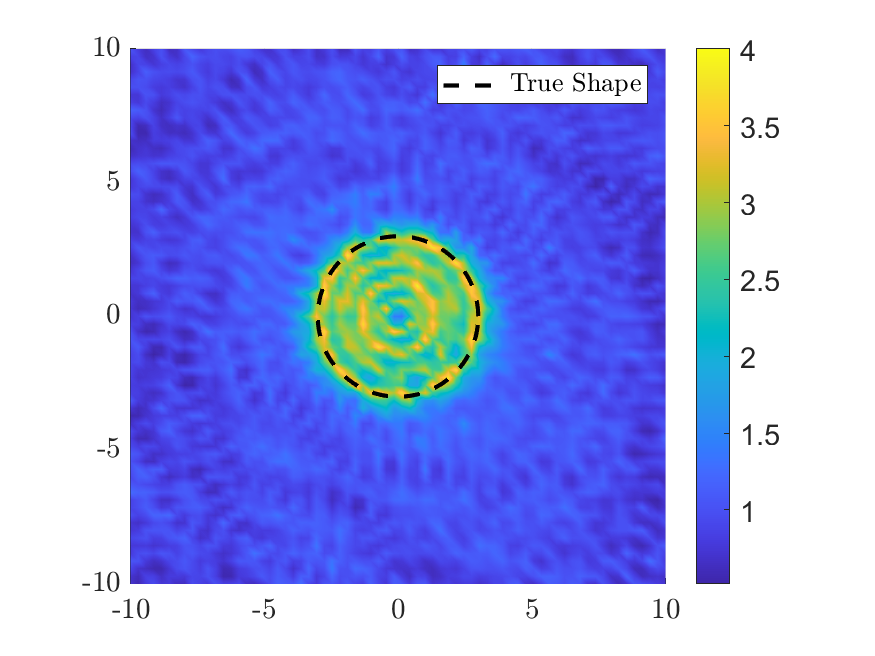
\includegraphics[width = \textwidth]{Numeric Simulations/Images/circle-20-noise-reconstructed}
						\caption{Circle with 20\% added noise.}
					\end{subfigure}
					\begin{subfigure}{.3\textwidth}
						\centering
						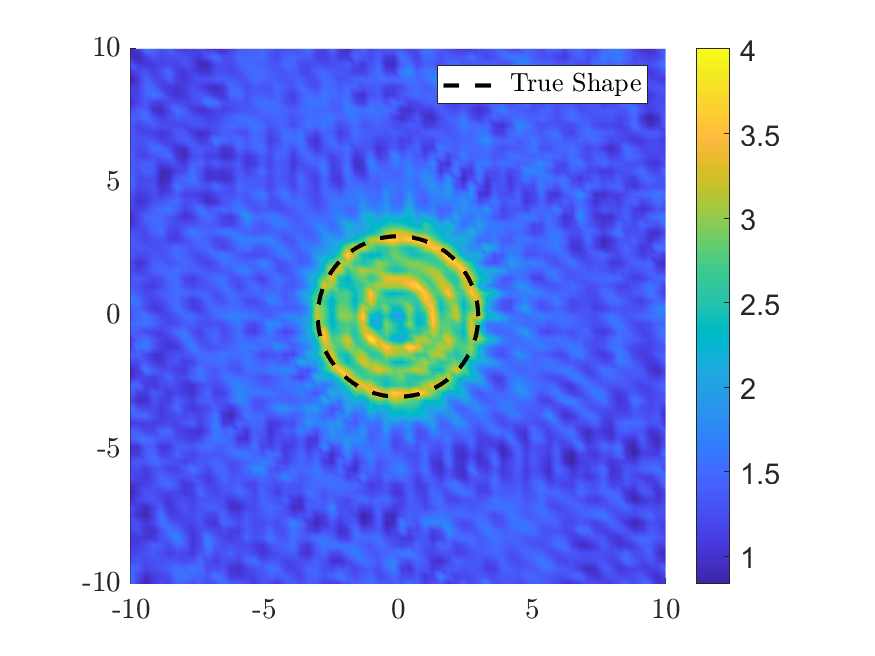
\includegraphics[width = \textwidth]{Numeric Simulations/Images/circle-40-noise-reconstructed}
						\caption{Circle with 40\% added noise.}
					\end{subfigure}
					\caption{Reconstructions of circular objects with various levels of noise in data.}
					\label{fig:circlenoise}
				\end{figure} 
				\begin{figure}[h]
					\centering
					\begin{subfigure}{.3\textwidth}
						\centering
						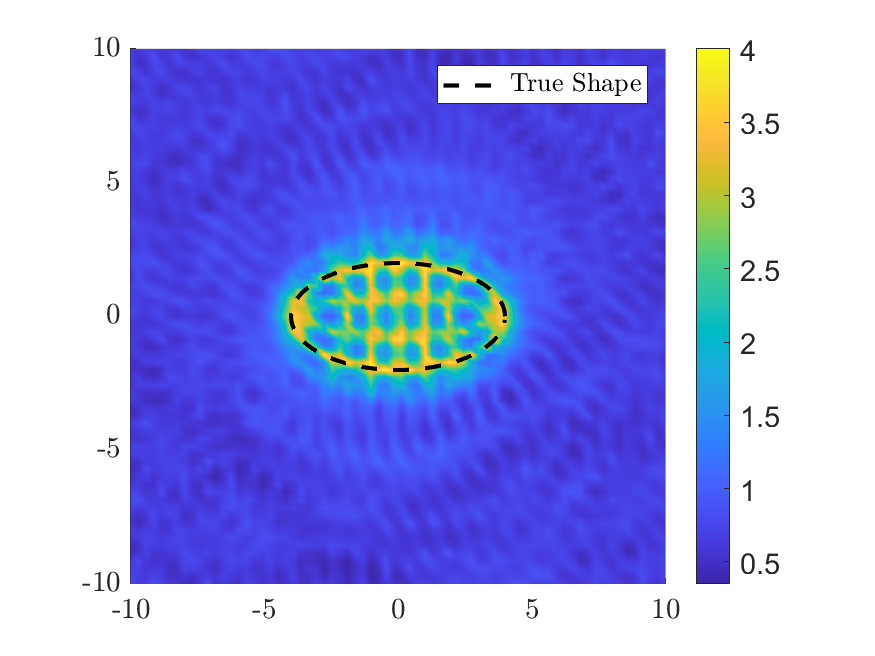
\includegraphics[width = \textwidth]{Numeric Simulations/Images/ellipse-10-noise-reconstructed}
						\caption{Ellipse with 10\% added noise.}
					\end{subfigure}
					\begin{subfigure}{.3\textwidth}
						\centering
						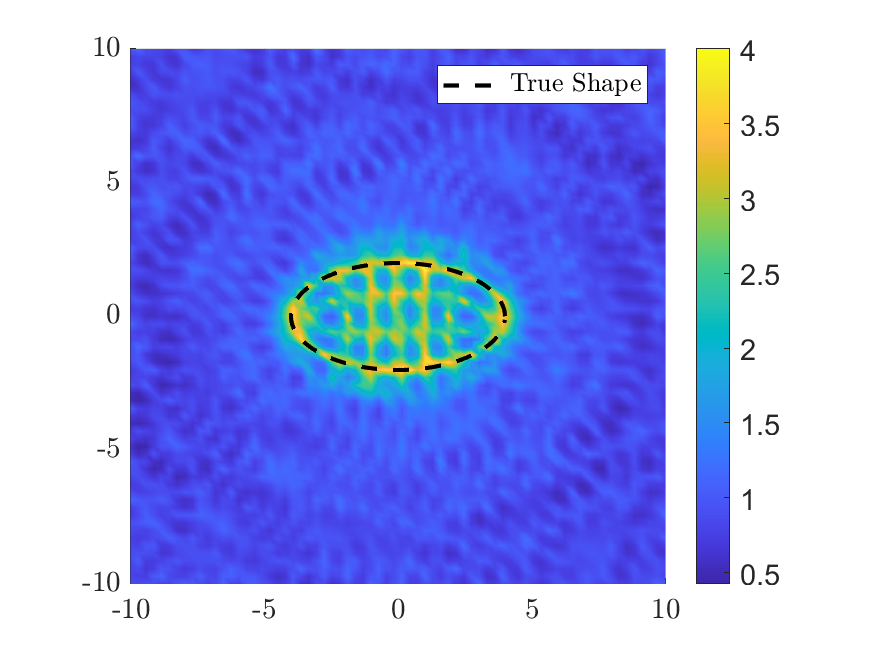
\includegraphics[width = \textwidth]{Numeric Simulations/Images/ellipse-20-noise-reconstructed}
						\caption{Ellipse with 20\% added noise.}
					\end{subfigure}
					\begin{subfigure}{.3\textwidth}
						\centering
						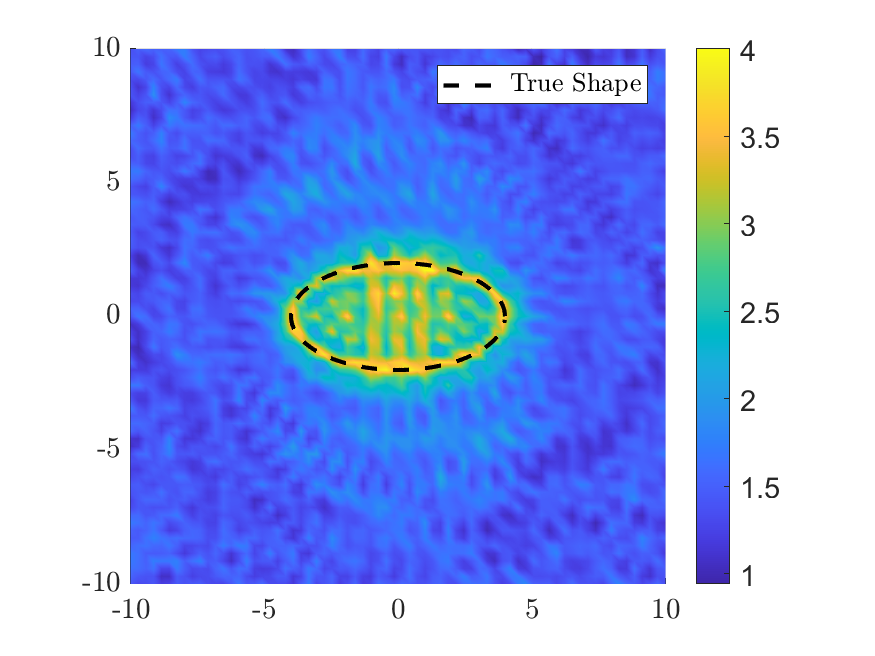
\includegraphics[width = \textwidth]{Numeric Simulations/Images/ellipse-40-noise-reconstructed}
						\caption{Ellipse with 40\% added noise.}
					\end{subfigure}
					\caption{Reconstructions of ellipses with various levels of noise in data.}
					\label{fig:ellipsenoise}
				\end{figure}
				\begin{figure}[h]
					\centering
					\begin{subfigure}{.3\textwidth}
						\centering
						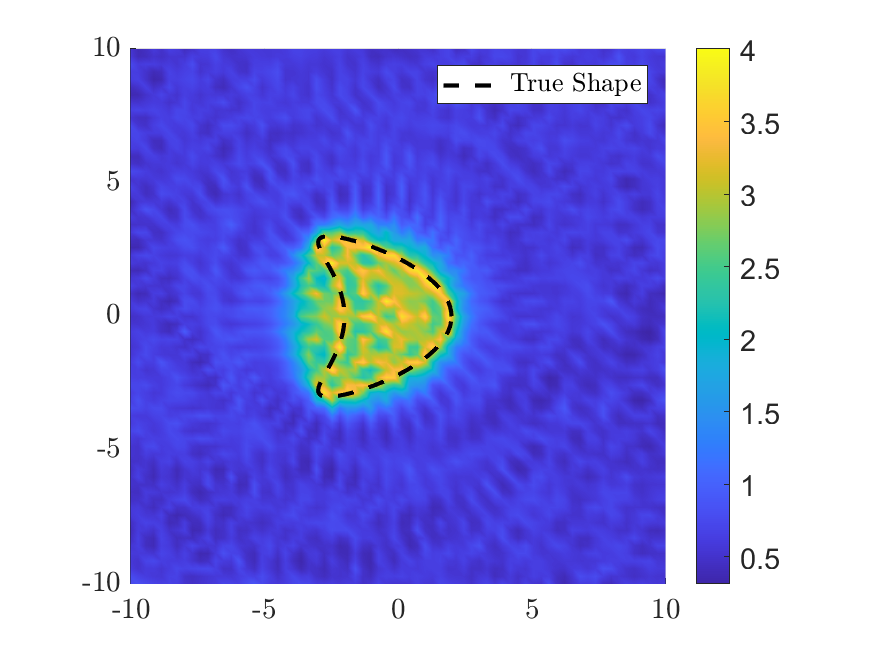
\includegraphics[width = \textwidth]{Numeric Simulations/Images/kite-10-noise-reconstructed}
						\caption{Kite with 10\% added noise.}
					\end{subfigure}
					\begin{subfigure}{.3\textwidth}
						\centering
						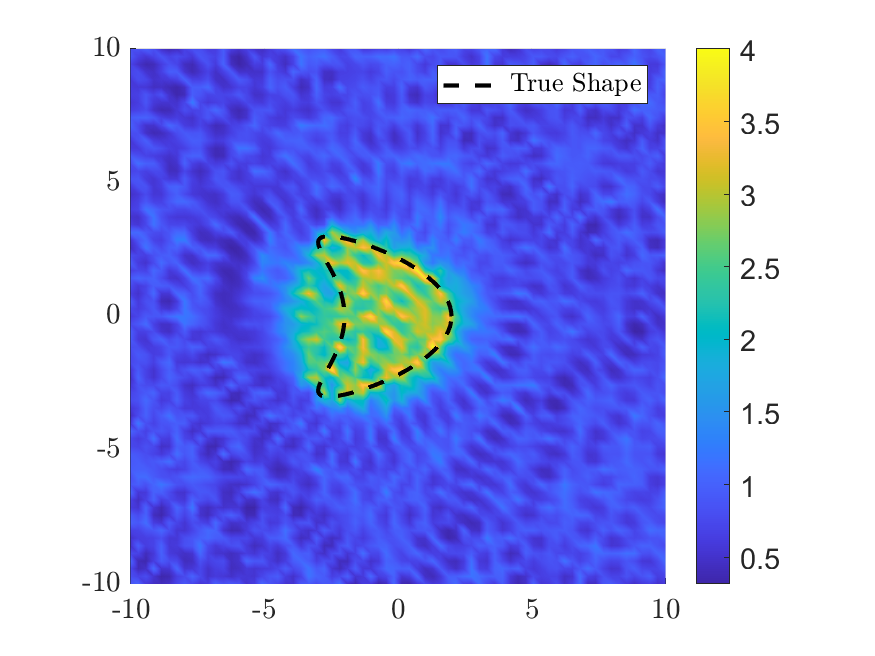
\includegraphics[width = \textwidth]{Numeric Simulations/Images/kite-20-noise-reconstructed}
						\caption{Kite with 20\% added noise.}
					\end{subfigure}
					\begin{subfigure}{.3\textwidth}
						\centering
						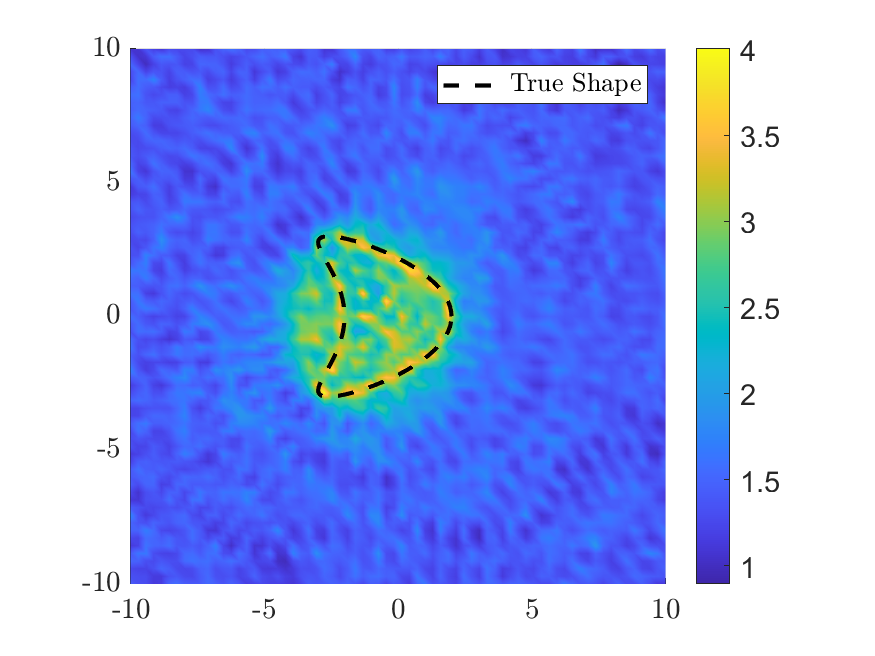
\includegraphics[width = \textwidth]{Numeric Simulations/Images/kite-40-noise-reconstructed}
						\caption{Kite with 40\% added noise.}
					\end{subfigure}
					\caption{Reconstructions of kites with various levels of noise in data.}
					\label{fig:kitenoise}
				\end{figure} 
		\printbibliography
			
\end{document}
